% CHAPTER 1
\chapter{Introduction}
\label{chp:1_introduction}

\section{Motivation and Problem Definition}
In recent years, deep neural networks have shown impressive performance in many vision related tasks such as image classification~\cite{he2015deep}, object detection~\cite{redmon2018yolov3} and image segmentation~\cite{long2015fully}. However, they are found to be vulnerable to intentionally crafted small perturbations called adversarial perturbations~\cite{szegedy2013intriguing}. These small perturbations added to the input image successfully change the output of a trained classifier by altering the logits large enough to change its decision to a preferred class~\cite{goodfellow2014explaining}. While these perturbations are optimized in \(\mathcal{L}_p\) spaces~\cite{carlini2017towards}, they are visible to human observers, since small \(\mathcal{L}_p\) does not always correspond to perturbations with less perceptual distortion~\cite{jordan2019quantifying,engstrom2018rotation}.

Since this intriguing property of neural networks has security implications in the production setting, it is often called \textit{adversarial attacks}. For example, some websites use CAPTCHAs (Completely Automated Public Turing Tests to Tell Computers and Humans Apart) to avert automated request agents such as web scrapers and spiders from automatically reaching their content. A widely used CAPTCHA type works by asking users select the images containing specific objects such as "bicycle" or "crossroad". A human can effortlessly detect the probed images while web scrapers would need to use classifiers such as DNNs to classify each image and select the correct ones. Such image based CAPTCHAs distort the visual content so that automated CAPTCHA solvers would fail the test, while the content could still be recognized by humans. To do this, recent CAPTCHAs has extended this setup by adding adversarial perturbations to the provided images to prevent DNN classified based solvers from automatically selecting the correct images. In Figure \ref{fig:googlecaptcha}, a recent CAPTHCA from Google is shown where the user is asked to select the images that contains "cars". Normally, a trained DNN could be used to classify images and to select the images whose output is the class "car" to pass the test. However, when these images are inspected, it could be seen that there is a noticeable adversarial noise added to the images to fool the DNN and to prevent the attacker from passing the test. When the amount of the additive noise gets high, it starts to become more difficult for humans to recognize the images, which is an undesirable side effect, and this negatively affects the usability of CAPTCHAs.
\begin{figure}[t]
    \centering
    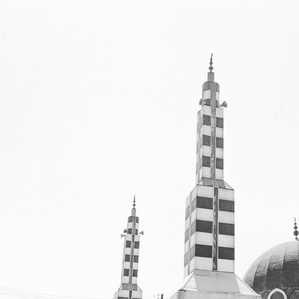
\includegraphics[width=0.4\linewidth]{captchas/1.png}
    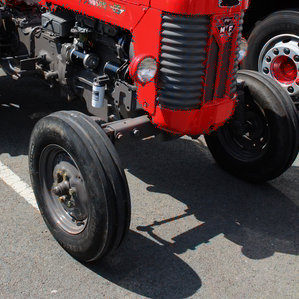
\includegraphics[width=0.4\linewidth]{captchas/2.png}
    \caption[Adversarially perturbed visual CAPTCHA examples.]{ Two CAPTCHA examples from Google where adversarial examples are used to prevent web scrapers and spiders that are using automatic image classifiers such as DNNs by adversarially perturbing the CAPTCHA images.}\label{fig:googlecaptcha}
\end{figure}

Multimedia compression standards have been developed to compress visual media such as images and videos to reduce the amount of data with minimum amount of distortion on the perceived output. One of the most fundamental findings about human vision that most lossy visual multimedia compression methods utilize is that human vision is much less sensitive to the spatial information and resolution loss in chrominance (color) than the luminance (intensity)~\cite{vorobyev2004ecology}. This observation is utilized in image compression as a technique known as ``chroma subsampling''. There are variants of chroma subsampling that only subsamples chrominance along horizontal axis (4:2:2) or both horizontal and vertical axes (4:2:0). Without further compression, (4:2:0) chroma subsampling reduces the size of an image effectively to half of its original size. Replacing the chroma components of the pixels in by neighboring chroma components does not yield visible artifacts.
%\section{Proposed Methods}
We employ these observations to derive a new type of adversarial attack based on spatial transformations in chroma channels of perceptual colorspaces. We apply spatial transformation only to the chroma components of input image while keeping the luminance component intact. Figure~\ref{fig:flowtochannels} shows the effect of a randomly initialized flow field applied to the luminance, chrominance and both set of channels. It is clear that spatial transformation in luminance channels causes visible distortions while chrominance only spatial transformations cause very subtle changes for human vision. This effect is much more highlighted when only the differences are observed after applying a flow field. Figure \ref{fig:diff} shows the absolute pixel difference from the initial image when the same flow field is applied to RGB, \(C_{b}C_{r}\) and a*b* channels, respectively.

\begin{figure}[t]
    \centering
    \begin{subfigure}[b]{.30\linewidth}
        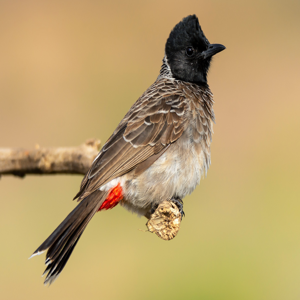
\includegraphics[width=\linewidth]{img.png}
        %        \caption{Original}
        \caption{}
    \end{subfigure}
    \begin{subfigure}[b]{.30\linewidth}
        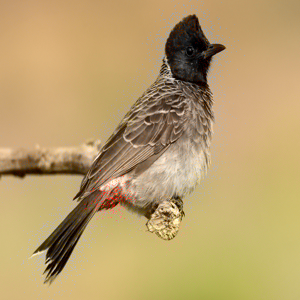
\includegraphics[width=\linewidth]{flowed_cbcr.png}
        %        \caption{Flow to CbCr channels}
        \caption{}
    \end{subfigure}
    \begin{subfigure}[b]{.30\linewidth}
        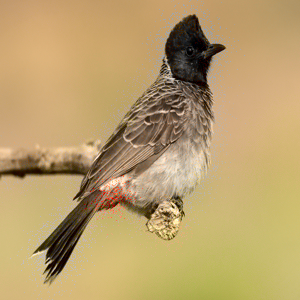
\includegraphics[width=\linewidth]{flowed_ab.png}
        %       \caption{Flow to \(a^*b^*\) channels}
        \caption{}
    \end{subfigure}
    \begin{subfigure}[b]{.30\linewidth}
        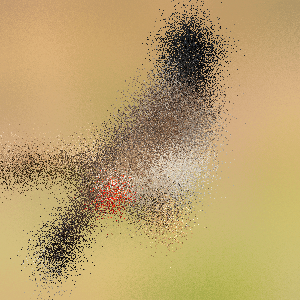
\includegraphics[width=\linewidth]{flowed_rgb.png}
        %      \caption{Flow to RGB channels}
        \caption{}
    \end{subfigure}
    \begin{subfigure}[b]{.30\linewidth}
        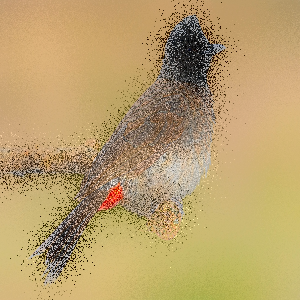
\includegraphics[width=\linewidth]{flowed_y.png}
        %     \caption{Flow to Y channel}
        \caption{}
    \end{subfigure}
    \begin{subfigure}[b]{.30\linewidth}
        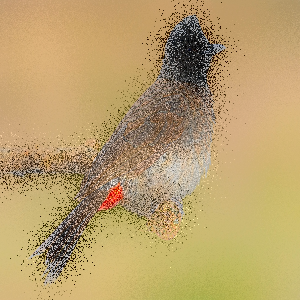
\includegraphics[width=\linewidth]{flowed_l.png}
        %\caption{Flow to L channel}
        \caption{}
    \end{subfigure}
    \caption[Effect of flow field applied to different channels]{Effect of flow field applied to different channels, (a) original image, Images where flow field is applied to (b) \(C_{b}C_{r}\), (c) \(a^*b^*\), (d) RGB, (e) Y and (f) L channel. The magnitude of the flow is scaled up to emphasize the effect for illustration.}\label{fig:flowtochannels}
\end{figure}

\begin{figure}[t]
    \centering
    \begin{subfigure}[b]{.4\linewidth}
        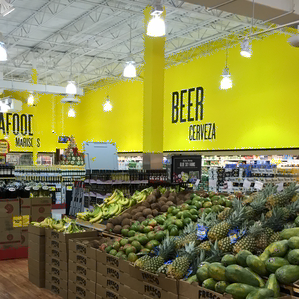
\includegraphics[width=\linewidth]{diff/209_lab_adv.png}
        \caption{}
    \end{subfigure}
    \begin{subfigure}[b]{.4\linewidth}
        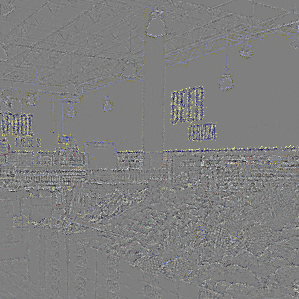
\includegraphics[width=\linewidth]{diff/209_rgb_diff.png}
        \caption{RGB}
    \end{subfigure}
    \begin{subfigure}[b]{.4\linewidth}
        
\includegraphics[width=\linewidth]{diff/209_ycbcr_diff.png}
        \caption{a*b*}
    \end{subfigure}
    \begin{subfigure}[b]{.4\linewidth}
        
\includegraphics[width=\linewidth]{diff/209_lab_diff.png}
        \caption{CbCr}
    \end{subfigure}
    \caption[Visual difference from random flow field application to different channels.]{ Visual difference from random flow field application to different channels, (a) original image, Visualization of pixel differences where flow field is applied to (b) RGB, (c) \(C_{b}C_{r}\), (d) \(a^*b^*\) channels. The magnitude of the flow is scaled up and contrast of the pixel differences is increased to increase the visibility for illustration. }\label{fig:diff}
\end{figure}


\section{Contributions of the Study}

The main findings of this thesis is published in a paper~\cite{aydin2019imperceptible} and the subject matter is further extended and elaborated in this thesis. The contributions of this work can be summarized as following;
\begin{itemize}
    \item Utilization of the findings of human vision and ideas from image and video compression to make imperceptible changes on images without any explicit \(L_p\) norm restriction.
    \item A novel method to generate adversarial examples with little to no perceptual distortion by applying spatial transformations in chroma channels of perceptual colorspaces optimized by widely used gradient-based optimizers without requiring any regularization term in the loss function.
    \item Modification of the proposed method to restrict the flow magnitude to have subpixel spatial drifts to further improve perceptual quality with a performance trade-off.
    \item Colorfulness analysis of NIPS2017 Adversarial Challenge dataset and effect of the colorfulness of input image to the performance of proposed methods.
\end{itemize}

\section{Organization of the Thesis}
This thesis is organized as follows. Chapter \ref{chp:1_introduction} provides an introduction on the thesis topic, explaining the motivation, defines the problem and briefly explains the methods and contributions of the thesis. Chapter \ref{chp:2_literature} mentions the literature about the thesis topic, presents the types and classifications of adversarial attacks and methods for generating imperceptible types of adversarial attacks or methods to improve perceptual quality of adversarial examples. Chapter \ref{chp:3_methodology} explains the methodology of the method proposed in this thesis in a detailed manner. It starts with spatial transformations, then explains spatially transformed adversarial examples and colorspaces to build the foundation of this thesis. Then, it explains the method proposed in this thesis. Chapter \ref{chp:4_results} mentions the setup of the experiments and presents the experimental results as well as analysis of numerical results from the experiments with a brief discussion. Chapter \ref{chp:5_discussion} provides a detailed discussion about the results presented in Chapter \ref{chp:4_results}, explains and discusses the implications of the findings and mentions the failure cases, discussing the possible reasons and potential remedies. Chapter \ref{chp:6_conclusion} draws conclusions on the thesis along with possible future studies of the new research questions with the thesis.
